\chapter{Aspects of scientific computing}\label{ch:computer}

The focus of these research notes is on LFT, which employs programming heavily.
In particular the computationally demanding MCMC code we write spurs us to
write code that is
\begin{enumerate}
  \item easy to read,
  \item well organized,
  \item future-proof, and
  \item high performance.
\end{enumerate}
Furthermore we must carry out statistical analysis of observables measured on
configurations produced by this MCMC code. In this chapter we collect
some information on these topics.


\section{Object-oriented programming}\label{sec:oop}


The first programming language I used for serious scientific calculations
\index{object-oriented programming}
was Fortran. Fortran does not traditionally 
allow\footnote{Actually I think more modern Fortran compilers 
allow for OOP, but I get the impression that C++ is the preferred language
in scientific computing for this.} for object-oriented programming (OOP); 
instead, very roughly, Fortran only
allows for two things:
\begin{enumerate}
  \item arrays or variables of some kind, along with 
  \item some functions that map them into each other.
\end{enumerate}
Actually programming in Fortran is kind
of a physicist's dream: it is very direct, and you can see exactly what
operations the computer is going to carry out. I will call Fortran
a {\it non-OOP} language.

An OOP language is more general than this, and hence it is a bit more powerful.
\index{compile time}\index{run time}
For the following discussion, it is useful to introduce two terms,
{\it compile time}, which is the time during which the code you wrote
is turned into an executable, and {\it run time}, which is the time during
which the executable runs.
Again very roughly, an OOP language has instead three things:
\begin{enumerate}\index{object}\index{function!OOP}\index{method}\index{class}
  \item {\it objects}, which I will define as any runtime entity that 
        takes up memory and has an address;
  \item {\it functions} or {\it methods}, which map objects to other
        objects; and
  \item {\it classes}, which are an abstraction of objects and/or functions,
        that do not take any space in memory or have an address. One common
        way to think of classes is as ``blueprints" for objects.
\end{enumerate}

Ultimately an important goal of OOP is to try to make your code more closely
mirror how things look in the real world, and maybe you can see that this
goal is more readily accomplished under this paradigm.
For example in point (1), you can see that variables
and arrays were generalized to objects. This gives you more flexibility in
coding, in case the real-world object you are thinking of is not easily
imagined as a variable or an array. The way that we invent these objects
is through point (3), the class. In addition to defining objects, the
class is an important organizational tool, allowing you to collect all
objects and functions that are related to some general idea,
which\index{encapsulation}\index{abstraction} is sometimes called 
{\it encapsulation}. Both functions and classes
are useful to hide implementation details from the programmer, minimizing
the what the programmer needs to provide to the program, which is
sometimes called {\it abstraction}.

Encapsulation and abstraction are useful to programmers in part because
they make the code much more readable (again because what you are typing
more closely resembles how you think of things in the real world) and
reduce code duplication (which prevents you from having to maintain
several duplicates). Furthermore you
can change the implementation details of that class
without having to modify anything that utilizes it. The drawback is that
it can be difficult to see precisely what operations the computer
performs. In my experience, this trade-off is hugely worthwhile, and I think
most modern software developers would agree.


\subsection{OOP in C++} 
Probably the best way to learn is through an example. To see the basics
of OOP in action, we will implement a \ff{CAT} class, and 
introduce some new OOP jargon and concepts along the way.
The example code, shown in Listing~\ref{lst:CATclass}, 
definitely works for C++14~\cite{cppDocumentation},
but it likely also works for earlier standards.
The first function we define, \ff{narrate}, is not part of the class;
actually it is there to make it easier to print to screen, which is
an example of abstraction. We see that it made the code easier to
read and reduced duplication.

\begin{code*}
\mycodeSnippet{c++}{exampleCode/cat.cpp}{1}{47}
\caption{Basic example of a class, the \ff{CAT} class, along with
a \ff{narrate} auxiliary function. The constructor appears on line 15,
and defines all the actions that should be taken when this object
is created. The destructor is indicated with a \ff{\~} and is defined
on line 22.}
\label{lst:CATclass}
\end{code*}

The \ff{CAT} class begins with the \ff{public} keyword, which
is a statement about accessibility. Anything that falls under the
\ff{public} heading can be used outside of the class\footnote{The other
two possibilities are \ff{private} and \ff{protected}. 
Anything under the \ff{private} heading
can only be seen by the class itself, while \ff{protected} members can be accessed 
by the class itself, as well as any derived classes that inherit from the class.
In C++ one can also define a \ff{struct} instead of a \ff{class}.
In a \ff{struct}\index{struct} the default access level is \ff{public} instead
of \ff{private}.}. 
Everything in the class falls
under this heading in this example. The first group of three lines
are variables stored inside the \ff{CAT} class; such variables
\index{attribute}\index{constructor}\index{destructor}\index{method}
are called {\it attributes}. The next group of two functions are
the {\it constructor} and the {\it destructor}, which I will explain
shortly. Finally the last group of four \ff{void} functions are 
called {\it methods}. It is basically correct to think of a class as a
collection of attributes and methods acting on them.

\begin{code*}
\mycodeSnippet{c++}{exampleCode/cat.cpp}{49}{61}
\caption{Main C++ code where the \ff{CAT} class is used.}
\label{lst:CATmain}
\end{code*}

To understand the constructor and destructor, let us turn to our main
code where we will use this class, shown
in Listing~\ref{lst:CATmain}. The output of this code is
given in Listing~\ref{lst:CATout}. In the first line of
the main, we declare a
\ff{CAT}-type\footnote{A {\it type}\index{type} is a category of data
defined by some properties or characteristics. The type often defines the sorts
of operations that one can do with that datum. For instance, integers, floats,
strings, and objects are all types. Types are related to classes but not exactly
the same. A class in particular tells you how something should be implemented,
whereas a type does not necessarily. For instance you might have a \ff{CAT}
type. Two possible \ff{CAT}-type implementations could be, e.g.
\ff{MEANCAT} or \ff{WUNKUSCAT} classes.} object, which we call \ff{cat}. 
We say that we have
{\it instantiated} \ff{cat}, and \ff{cat} is an {\it instance}
\index{instantiation}
of \ff{CAT}. \ff{CAT} is a class; therefore, as mentioned
earlier, it takes up no memory and has no address associated to it.
On the other hand, \ff{cat} is an object, and hence has some
memory associated to it at runtime. More precisely, it uses the
amount of memory required to hold its attributes.

The constructor is the function that is called every time an object is
instantiated. If you look back at the \ff{CAT} class, you can see that
the constructor takes an argument called \ff{name}. In the main,
the string ``Chooky" is being fed into this argument. A constructor does
not have to take an argument, or even explicitly do anything, but often
it is useful to have a constructor set the attributes to some default values.
That is what the constructor does in this case, and it also tells the
user that it instantiated a \ff{CAT} object.

\begin{code*}
\mycode{text}{exampleCode/catOutput.txt}
\caption{Resulting output from main C++ code of Listing~\ref{lst:CATmain}.
This output reflects some of the automatic actions taken when \ff{CAT}
classes are instantiated and destroyed.}
\label{lst:CATout}
\end{code*}

The destructor is the function called every time an object is destroyed.
The two most common times an object is destroyed are when the object
leaves scope and when the program ends. Scopes in C++ are defined by
curly brackets \ff{\{\}}. So for example if you define a new variable
inside a function, and you only use this variable inside that function,
the {\it scope} of that variable is the inside of the function. 
Other examples of scope include
the inside of \ff{if} and \ff{while} statements and the
\index{scope}
insides of classes. In Listings~\ref{lst:scope} and \ref{lst:scopeOut}
we see constructors and destructors in action as the objects
leave scope. Note the order of creation 
and destruction.

\begin{code*}
\mycodeSnippet{c++}{exampleCode/scope.cpp}{40}{47}
\caption{An example main showcasing scopes in C++. Here,
Tallulah-Paige is in her own scope, set aside by
curly brackets. By line 44, we have left the scope with
Tallulah-Paige in it, and she is ruthlessly and
automatically exterminated by her destructor.}
\label{lst:scope}
\end{code*}
\begin{code*}
\mycode{text}{exampleCode/scopeOutput.txt}
\caption{Output for the main code of Listing~\ref{lst:scope}.
We see that Tallulah-Paige perishes before Ziggy is instantiated.}
\label{lst:scopeOut}
\end{code*}

This practice of objects automatically allocating memory through their
constructors and destroying themselves when they leave scope
sometimes goes under the name\index{resource acquisition}
{\it resource acquisition is initialization} (RAII).
This strategy helps avoid\index{memory leak} {\it memory leaks},
which is when the computer fails to release some unneeded 
memory\footnote{Failure to release memory can negatively impact performance;
for instance if you never release memory, then long and memory-intensive
programs will quickly use up all of a system's available memory.}.

Turning back to the main, we see that we can access attributes of
\ff{cat} such as \ff{\_name} directly, and we can also call
methods of \ff{cat} like \ff{speak()}. This is possible because
we made these public attributes and methods. Note that inside the class,
it is enough to use the attribute or method name by itself. Outside the
class, i.e. inside the main, we have to use the object as an 
intermediary.

Hopefully this is enough for you to get at least an intuition for
what OOP is, how it works, and why someone would want to use it. These
few pages are just the beginning; there are many more advanced
features available to C++ that make classes extremely generalizable.
Besides the advantages of being object-oriented, C++ also has many
features that make it valuable for high-performance computing.
For example you can manipulate exactly where and how objects
are stored in memory. There are lots of good references for OOP
in C++ out there, but a good start might be Ref.~\cite{tp:cpp}.\\

\subsection{OOP in Python}

We continue by discussing OOP in Python. 
You can find lots of useful
tutorials online, for instance here~\cite{pythonOOP}. We will use
Python3~\cite{python3}.

In this section we will demonstrate
a couple other important features of the OOP paradigm. In particular we will
discuss {\it inheritance},\index{inheritance} the process by which a
class (the {\it child}\index{child} class) inherits attributes and methods
from a more general class (the {\it parent}),\index{parent} and
{\it operator overloading}, \index{operator overloading} where one generalizes 
operators such as $+$ to function with objects of the class you defined.
Inheritance is useful organizationally as it helps you think of some class
as a special case of a more general class. Furthermore it reduces code
repetition, since the child has access to all methods and attributes defined in
the parent. Operator overloading enhances readability, for example by
helping your code more closely mirror mathematical notation.

\begin{code*}
\mycodeSnippet{python}{exampleCode/cat.py}{1}{36}
\caption{Example \ff{CAT} class in Python. Here \ff{MEANCAT}
inherits from \ff{CAT}.}
\label{lst:CATpython}
\end{code*}

Let us begin by implementing the \ff{CAT} class from before in Python,
which is shown in Listing~\ref{lst:CATpython}. One nice feature of Python classes
is the \ff{\_\_doc\_\_} attribute, which is set here as the first string
in quotes, giving a description of the class. Note also that Python
does not have the \ff{private} or \ff{public} distinction that
C++ has; indeed all attributes and methods in Python OOP are effectively 
public\footnote{You can obfuscate attributes by leading with a double 
underscore \ff{\_\_} so that it is not as easily accessible. Still, there 
are ways to access such attributes.}.
The constructor and destructor\footnote{Python does not treat scope the same
way as C++, so an object is not destroyed automatically when you e.g.
exit a \ff{for} loop. Automatic object destruction in Python 
happens through \index{garbage collection}
its {\it garbage collector}, for example when the program terminates,
or when an object loses its reference by being reassigned.} are identified with
\ff{\_\_init\_\_} and \ff{\_\_del\_\_}, respectively. All of
\ff{\_\_init\_\_}, \ff{\_\_del\_\_}, and \ff{\_\_doc\_\_} 
are examples of
Python special functions, which will be discussed in a bit more detail
when we get to operator overloading. 
Two more syntactical characteristics 
to point out are that methods always take the \ff{self}\footnote{The
\ff{self} keyword refers to particular instance which is using
the called method.} reference as 
the first argument, and that this reference is always required to
interact with class methods and attributes, even within the class itself.

\begin{code*}
\mycodeSnippet{python}{exampleCode/cat.py}{39}{65}
\caption{Main code using the \ff{CAT} and \ff{MEANCAT} classes.}
\label{lst:CATmain}
\end{code*}
\begin{code*}
\mycode{text}{exampleCode/pythonCatOutput.txt}
\caption{Output from the code of Listing~\ref{lst:CATmain}.}
\label{lst:CATout}
\end{code*}

To demonstrate inheritance, we consider a new kind of \ff{CAT}, a
\ff{MEANCAT}. \ff{MEANCAT}s prefer to hiss rather than meow, and
their \ff{speak()} method should reflect this behavior. Nothing else
about a \ff{MEANCAT} is different. To indicate that \ff{MEANCAT}
should inherit from \ff{CAT}, one just passes \ff{CAT} as an argument
in the class definition.
%\footnote{It is also possible for a class to inherit
%from more than one parent. This is called {\it multiple inheritance},
%\index{inheritance!multiple} and it can be accomplished in Python by passing
%multiple arguments to the definition, e.g. \ff{MEANCAT(CAT,MAMMAL)}.}
The redefinition of the \ff{speak()} method
in \ff{MEANCAT} overrides that of its parent, \ff{CAT}. One last
feature to point out is the use of the \ff{del} keyword, which lets you
call an object's destructor.
Some main code utilizing the \ff{CAT} and \ff{MEANCAT} classes
is given in Listing~\ref{lst:CATmain} along with the
corresponding output in Listing~\ref{lst:CATout}.

Finally we will have a look at operator overloading. For this example we
will create a rudimentary and wildly incomplete class for a simple math 
object of interest to high energy physics: the $\SU(2)$ matrix.
The code is shown in Listing~\ref{lst:SU2}.

\begin{code*}
\mycodeSnippet{python}{exampleCode/SU2.py}{1}{41}
\caption{Example $\SU(2)$ matrix class.}
\label{lst:SU2}
\end{code*}

Here the attributes are the elements of the matrix. 
I have opted to use double underscores \ff{\_\_} in front of
the attribute names. As mentioned in an earlier footnote, this hides the
attributes from the user as shown below.
Hiding these attributes is important for the \ff{SU2} class, because the
elements should always be \ff{complex}, and I want to make sure the
user cannot change the type. The \ff{complex} type is
enforced through the \ff{setElement} method.

\begin{code*}
\mycodeSnippet{python}{exampleCode/SU2.py}{45}{54}
\caption{Example main code utilizing the \ff{SU2} class
of Listing~\ref{lst:SU2}.}
\label{lst:SU2main}
\end{code*}
\begin{code*}
\mycode{text}{exampleCode/SU2Output.txt}
\caption{Output from Listing~\ref{lst:SU2main}.}
\end{code*}

To use operator overloading, each binary operator has a special function name.
In the \ff{SU2} class example, we overloaded the \ff{+} operator. Its special
function name is \ff{\_\_add\_\_}, and the two arguments are the LHS and
RHS of the operator, respectively. Python allows also for the overloading
of other algebraic operators, bitwise operations, and comparison operators.
In our example, we have edited the \ff{\_\_str\_\_} operator, which
controls how an \ff{SU2} object is printed to screen.
In Listing~\ref{lst:SU2main} we give some quick examples of 
this \ff{SU2} class in use. 
%Note that
%the \ff{=} sign here is not a copy constructor; instead both \ff{g} and
%\ff{h} are references to the same \ff{SU2} object. This means that
%if you change \ff{g}, \ff{h} will change as well. Be careful!


\section{Addressing storage challenges}

\index{binary}\index{binary!file}
The configurations that we generate store lots of information, and to make a
file human-readable costs extra storage space. Hence we must store
configurations as binary, to save space. Unfortunately for you,
this means you will have to learn in detail how a computer reads and writes data
to a machine.

\index{bit}\index{byte}
We start with the basics. A {\it bit} is the smallest unit of data a computer
can process or store. Each bit is represented as a 0 (false) or 1 (true).
Eight adjacent bits are organized into a {\it byte}.
Since the fundamental information unit has two possibilities, storage
sizes must exist in powers of two. For this reason, the naming scheme
for larger numbers of bytes is collected in powers of $2^{10}=1024$
instead of 1000 like it usually goes with the metric system.
In \tabref{tab:byte} we collect the tower of storage sizes
along with some references to get a feeling for how much information
they store. This whole two-bit numbering system is, as you probably
already know, called {\it binary}.

\index{byte!peta}
\index{byte!exa}
\index{byte!zetta}
\begin{table}
\centering
\caption{Converting bits to bytes.}
\begin{tabularx}{\linewidth}{lCLr}
\hline\hline
Name & Abbreviation & Bits & Information of...\\
\hline
kilobyte & KB & $1024$ & page of text \\
megabyte & MB & $1024^2$ & pop song MP3 \\
gigabyte & GB & $1024^3$ & computer game \\
terabyte & TB & $1024^4$ & laptop's storage \\
petabyte & PB & $1024^5$ & library of congress \\
exabyte  & EB & $1024^6$ & Google's storage capacity \\
zettabyte  & ZB & $1024^7$ & all data on internet \\
\hline\hline
\end{tabularx}
\label{tab:byte}
\end{table}

\index{hexadecimal}
Besides the binary numbering system another common system organizes things in
base 16. This is the {\it hexadecimal} system. Since we have only ten numerals,
this requires the introduction of some letters for its representation,
as shown in \tabref{tab:hexadecimal}. In C and C++ programming,
hexadecimal numbers are preceded by an indentifier \ff{0x} to
indicate that it's hexadecimal\footnote{Instead it is preceded
by \ff{0b} if it's binary.}.
Since hexadecimal is base 16, it follows that each hex digit is equivalent
to four bits. Hence the length of a hexadecimal number in C and C++
depends on the size of the object it represents. Finally, sometimes
a hexadecimal can be appended with a string like \ff{ull} to
indicate it represents an \ff{unsigned long long} object. 

\begin{table}
\centering
\caption{Converting decimal to hexadecimal.}
\begin{tabularx}{\linewidth}{CCCCCCCCCCCCCCCC}
\hline\hline
0 & 1 & 2 & 3 & 4 & 5 & 6 & 7 & 8 & 9 & 10 & 11 & 12 & 13 & 14 & 15\\
0 & 1 & 2 & 3 & 4 & 5 & 6 & 7 & 8 & 9 & a & b & c & d & e & f\\
\hline\hline
\end{tabularx}
\label{tab:hexadecimal}
\end{table}

In any such numbering system, numbers are represented with the least significant
digit in the right-most place. For example one has for decimal, binary, and
hexadecimal, respectively
\begin{equation*}\begin{aligned}
  \ff{11} &= 1\times10^1+1\times10^0, \\
  \ff{101} &= 1\times2^2+0\times2^1+1\times2^0,~\text{and} \\
  \ff{0xf0} &= 15\times16^1+0\times16^0.
\end{aligned}\end{equation*}
While this is the way humans read significant digits, how the computer stores
binary depends on a convention called the {\it endianness}.
The storage is {\it big endian} \index{endian!big} if the most significant digit 
is at the smallest memory address. Conversely the
{\it little endian} \index{endian!little} convention specifies the least
significant digit is at the smallest memory address\footnote{I guess the way
to remember this is whether the smallest memory address starts at the most
significant digit, i.e. the big end, or the other way around.}.

\index{bit!mask}
Sometimes you may encounter {\it bit masking}. The idea is that one compares
two binary numbers bit-by-bit, and new binary is created by a logical operator
applied to each bit. For example
\begin{equation*}
  \ff{001 \& 111} = \ff{001}. 
\end{equation*}

The above schemes give ways to represent data with numbers, but it is also
useful to understand how the data are stored physically in the system.
The {\it memory cell} is the most fundamental element of memory. In the old
days, a memory cell consisted of ferromagnetic material, shaped in a torus, with
a wire running through its hole. A current going through the wire induces a
magnetic field in the plane of the torus, aligning the spins either CW or CCW.
When the current stops, the torus keeps its magnetization due to 
{\it hysteresis}\index{hysteresis}. One bit is stored in this cell, which is 0
or 1 depending on the magnetization direction.

Nowadays it is more common to use semiconductor memory. The cell in
semiconductor memory is a small circuit consisting largely of transistors.
Certain transistor setups allow charge to be trapped inside of them,
which one can interpret (depending on your convention) as a 0-bit. The state
without trapped charge would the be interpreted as a 1-bit.
For memory that is only needed in the short term, the bit can be implemented 
instead as a full or discharged capacitor.

Now we have some intuition how data is generally stored on a computer.
The physical location of the memory units that will be utilized by your
program are represented in the lowest-level software, i.e. the software
directly managing the computer hardware, as a {\it physical address}\index{address!physical}.
At the same time, your computer has its own representation for the physical
memory, which is the {\it virtual address}\index{address!virtual}.
Back in the day, physical and virtual addresses more or less directly corresponded.
Nowadays the mapping between physical and virtual addresses is stored inside a
data structure called a {\it page table}\index{page table}.
This is roughly what is under the hood of the memory
addresses\index{address!memory} discussed above.

Next we discuss some strategies for accessing computer memory.
A {\it stack operation}\index{stack} is a type of computer operation involving a 
collection of data items called a {\it stack}. In a stack operation, data can be 
pushed (added) onto the stack and popped (removed) off the stack. It can be thought 
of as a type of Last-In-First-Out (LIFO)\index{LIFO} data structure.
Other possibilities include queues, trees, graphs, and hash tables.


\begin{figure}
\centering
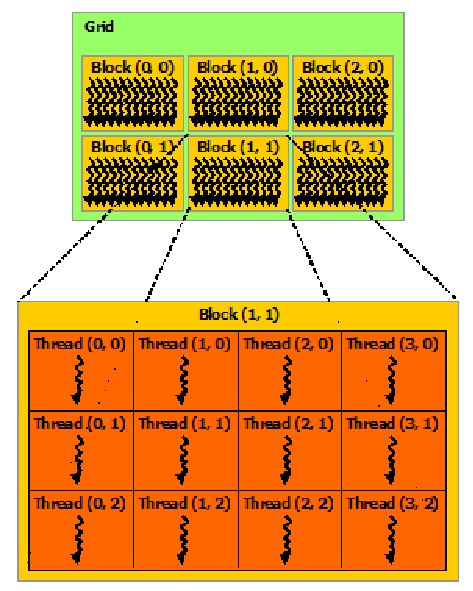
\includegraphics[width=0.6\linewidth]{figs/threadBlock.pdf}
\caption{The thread/block hierarchy used in NVIDIA GPUs.
Image taken from Ref.~\cite{NVIDIA}.}
\label{fig:threadBlock}
\end{figure}


\section{Improving performance}

For pure $\SU(2)$ simulations like what I did in grad school, 
it may take months (or years!) for a single-processor MCMC simulation to
generate enough data to get reasonable error bars. In order to get
results in time to finish a PhD thesis, it is necessary to consider ways to
optimize the code.

When getting into details about coding specifically, this section tends to focus
on C++ and Python. Besides being two languages with which I'm comparatively
familiar, they are also popular choices for scientific computing. When GPU
parallelization is mentioned, we discuss NVIDIA, although alternatives like AMD
and Intel exist nowadays.

\subsection{Parallelization}

A common strategy is to divide the lattice into smaller sublattices, updating
simultaneously on each sublattice, passing relevant information between the
sublattices whenever necessary. {\it Parallelizing}\index{parallelization} 
in this way offers a speed
up factor somewhat less than the number of sublattices used. A standard way to
parallelize code is to use the Message Passing Interface (MPI). MPI\index{MPI} 
is a library that allows for efficient exchange of information between processors 
and can be included in Fortran, C, and C++ programs.

One way to approach parallelism is called Single Instruction Multiple
Data\index{SIMD} (SIMD). In this approach, the same instruction is given to
multiple data elements. For instance the first way you learn implement scalar
multiplication for a vector is through a simple loop:
\begin{verbatim}
do from i=0 to i=ndim
  v[i] *= 2
end do
\end{verbatim}
Instead of saying ``perform this multiplication, now perform the next one", SIMD
says to perform all the multiplications simultaneously, at least in the ideal
case. Sometimes this approach is referred to as {\it
vectorization}\index{vectorization}.

To get a quantitative understanding of performance, one introduces
the {\it clock cycle},\index{clock cycle} which is the smallest unit of
time in a computer\footnote{Most CPUs keep time using a quartz crystal.
The basic idea is that an electric field will cause the quartz to
vibrate. The frequency of this vibration is the clock cycle.
This frequency can be tuned according to the shape and size of the
crystal, as well the placement of electrodes on it.}.
In the olden days, only one computation would be carried out per cycle;
nowadays it is more common to carry out many. The number of
computations per clock cycle is known as the\index{clock speed} {\it clock speed}.

A CPU\index{CPU} is divided into several\index{core} physical {\it cores}, each of which can
carry operations separately. This is then one way to carry out parallelization:
You use MPI to have each core execute different tasks simultaneously.
A virtual entity comprising of these tasks being executed on one core
is usually called a\index{thread} {\it thread}. Sometimes one core splits
tasks between two threads. For pure $\SU(2)$ calculations, this
is sufficient.

We will see in \chref{ch:ferm} that simulations with dynamical fermions
are much more complex, and correspondingly, they are much more
computationally intensive. For such purposes, it is not really ideal even
to use CPUs. It was realized in the 2000s~\cite{egri_lattice_2007}
that\index{GPU} GPUs, which
are often needed for the numerous calculations required to render graphics
in video games, could be adapted for use in lattice QCD calculations.
In a GPU, there are many (often thousands) of cores, which allows for
extremely high parallelization. On a single GPU, no MPI is required;
however GPUs have memory limitations, such that they may not always accommodate
a single lattice, and in such cases MPI can be used to link
multiple GPUs together\footnote{How you link GPUs together depends on the
system you run on. Usually communication between GPUs is the slowest part
of a calculation, so one may utilize other frameworks besides MPI, usually
depending on the GPU manufacturer, to get a performance boost.}.
Since there are so many cores, it is practical to introduce an organizational
hierarchy. The most common is used by NVIDIA, where threads are collected
into\index{block} {\it blocks}; this is shown in \figref{fig:threadBlock}.

\subsection{Evaluating performance}

Lattice projects studying physically realistic setups
 are extremely computationally demanding; for instance
a recent HotQCD study utilized ensembles that required
$\order{2000}$ GPU-years of compute time and take up 2.4 PB of storage 
space~\cite{Bollweg:2021vqf}. Meeting these computational demands is
not cheap, and it is no longer sufficient to simply foist your
calculation onto GPUs. For these applications, it becomes crucially 
important that your code is highly
optimized to get the most bang for your buck.
We will now review some key concepts and terminology
relevant to assessing the performance of code
in high-performance computing\index{high-performance computing} (HPC). 

In this context, it is useful to define a few terms. A floating
point operation\index{FLOP} is a calculation of floating point arithmetic. In a
scientific context, this type is very common, so FLOPs are a good indicator
of the amount of arithmetic a code is doing. Any scientific code you write will
be in effect processing data. The rate at which data is processed
is called the {\it throughput},\index{throughput} 
and it can be measured in, for instance, FLOPs
per second, sometimes indicated\footnote{Please take care not to
mix up FLOPs with FLOP/s.} FLOP/s. The rate at which data is
transferred is called the {\it bandwidth},\index{bandwidth}
which can be measured in bytes/s.

\begin{figure}[t]
  \centering
  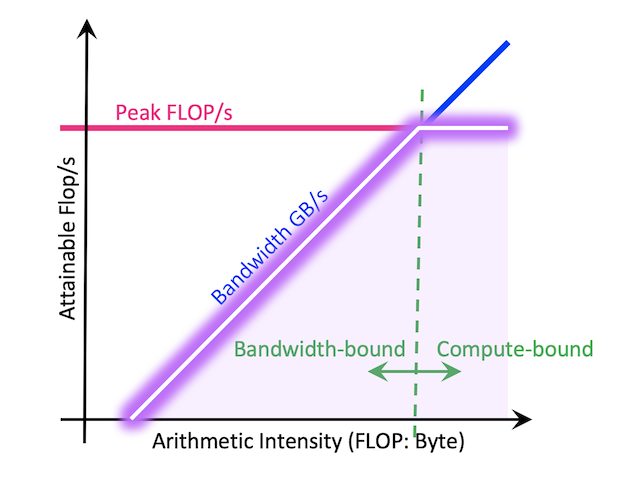
\includegraphics[width=\linewidth]{figs/Roofline-intro.png}
  \caption{Schematic example of a roofline analysis.
           Image taken from Ref.~\cite{roofline}.
           The light purple line indicates the theoretical
           maximum performance under this model.}
  \label{fig:roofline}
\end{figure}

\index{roofline performance analysis}
Obviously performance is limited by the hardware carrying out a calculation, for
instance the CPU, but it is also limited by the rate at which things are loaded
and extracted from memory. The {\it roofline performance model} is an elementary
way to see where your code stands with respect to these two limitations.

The {\it arithmetic intensity}\index{arithmetic intensity} of some code is
\begin{equation}
  \text{AI}=\frac{\text{\# FLOPs}}{\text{data movement in bytes}},
\end{equation}
where the numerator represents the number of FLOPs needed by that code, and the
denominator represents how much data you need to move in bytes in order to
support those FLOPs. From this equation it's clear that the attainable
FLOP/s scales linearly with arithmetic intensity.

Fig.~\ref{fig:roofline} shows a sketch of this model. The vertical
dashed line gives the {\it machine balance point}.\index{machine balance point}
This analysis is useful to try to diagnose whether one should look into
memory efficiency or algorithm improvement to try to speed up the code.
Code in the purple region to the left of the machine balance point
tends to be limited by bandwidth.

When it comes to evaluating the performance as one increases the number
of GPUs, a straightforward approach is to simply plot throughput against
the number of devices. In this context, one may be interested in
{\it strong scaling}\index{scaling!strong}, which measures the effectiveness 
of a parallel computing system when the problem size\footnote{In the context
of LQCD, the problem size is usually proportional to the lattice size
$N_\sigma^3\times N_\tau$.} remains constant, 
but the number of processing elements (cores, nodes, etc.) is increased.
In the ideal case\footnote{We never achieve the ideal case because of,
for instance, communication overhead.}, throughput
increases linearly with the number of processing elements.
One can also investigate {\it weak scaling}\index{scaling!weak},
which evaluates the performance when both the problem size and the number 
of processing elements are increased proportionally. 
Hence for a weak scaling test, the work assigned to each processing element 
remains fixed as new resources are added. Like with strong scaling,
perfect weak scaling would suggest throughput increases linearly with
the number of processing elements. In practice, it is much easier to
get closer to ideal weak scaling. There can be many reasons
for this, but a major one is that if the number of processors becomes
comparable to the number of computations, the code will spend a significant fraction
of the time communicating, which is hugely inefficient. Hence weak scaling is
usually a more relevant performance metric. 


\subsection{Optimizing memory usage}\label{sec:memory}

If you find your code is bandwidth-bound, there are a number of strategies that
can be used to improve performance. One way is to reshape your algorithm so that
it requires less communication. This can be quite challenging. An easier way is
to look in detail where your memory is being stored. Modern computing
architectures have multiple levels of memory, organized in the following by
increasing distance from the processor:
\begin{enumerate}
  \item {\it Registers}\index{register} are located inside of the processor
itself. They hold very little data but are extremely fast.
  \item {\it Caches}\index{cache} are also located inside the processor.
Actively used data from the main memory, which we will discuss next, is duplicated
in the cache for faster access. A processor can contain a cache hierarchy, for
instance many GPUs have L1, L2, and L3 caches, which in that order become
gradually larger but slower.
  \item {\it Main memory}\index{memory!main} is no longer inside the processor,
but has a comparatively large storage size. It is connected to the processor
via a {\it bus}\index{bus}. On circuit boards, you can sometimes see the 
connections as thin lines of a metal, such as copper, called {\it
traces}\index{trace}. The bus also requires logical units made of transistors
that manage the this transfer between devices.
Usually there are multiple buses connecting the main
memory with the processor, for instance one bus may send a number that indicates
the desired location of the data. This number is the {\it memory address}.
Another bus will then transfer the data themselves.
\end{enumerate}
As already hinted in some of the above discussion, as one increases physical
distance from the processor, the latency tends to increase, or conversely the
bandwidth decreases. This increase in latency has many causes, the easiest of
which to understand are:
\begin{enumerate}
  \item Memory addresses correspond to physical locations on the storage device.
Reading and writing data is implemented through some physical operation at that
physical location, and hence you may lose time if you need to change locations,
depending on how this is implemented. Registers and caches let you carry out
repeated operations on a section of your full memory, limiting latency of this kind.
  \item Coordinating data transfer requires instructions to be sent around. The
further away the memory is, the more complicated it is to access that memory,
and hence the more instructions are required. And of course it takes time to
process instructions.
\end{enumerate}

\section{C++ best practices}

As discussed in the last section, achieving optimal performance is challenging
and subtle. When writing a lattice code, it is therefore crucial to choose
a language that
\begin{enumerate}
  \item gives the programmer control over technical details like how hardware
interactions are handled and how memory is stored; and
  \item allows the programmer to write code that is highly readable and
easy to use, so that the code can continue to be used and maintained
for a long time.
\end{enumerate}
These two requirements rule out almost every language except C++, which has
become the de facto standard for high-performance LQCD code\footnote{For
instance the two most widely-used code bases, Grid and QUDA, are both
written in C++. \simulat, which I work on, is also written in C++.}.
In the interest of point 2 above, it is worthwhile to discuss some
best practices in C++ programming.

When making new classes, one often has to think how memory should be allocated
and deallocated, in particular when defining constructors. The {\it rule of
three}\index{rule of three} states that whenever a type needs one of the
following, it needs all three:
\begin{itemize}
  \item copy constructor,
  \item copy assignment,
  \item destructor.
\end{itemize}
A common example where this is especially important is when your destructor 
explicitly deallocates some memory. If no user-defined copy constructor exists,
C++ implements a {\it shallow copy}\index{copy!shallow}. A shallow copy of an
object shares some of the same data as the original object, such as a 
pointer\footnote{By contrast, a {\it deep copy}\index{copy!deep} will create
an entirely new object with its own data.}.
Hence changing the attribute of a shallow copy will also change the attribute of
the original. This means that when the destructor is called on a shallow copy,
it will deallocate the original copy's data, and hence when it comes time for
the original copy to deallocate, there is nothing left!
This leads to {\it undefined behavior}\index{undefined behavior}, which is sort
of a catch-all term for a result of compiling and running that cannot be
predicted\footnote{When doing parallel computing, a commonly encountered type of
undefined behavior is a {\it race condition}\index{race condition}. 
This happens whenever two
processes try to write into the same chunk of memory at the same time. In my
experience, undefined behavior due to a race condition may not even produce the
same results after two runs of the same compilation.}. Compilers will not always
catch undefined behavior; hence it's safest to just use the rule of three from
the beginning.

An extension to the rule of three is the {\it rule of five}\index{rule of five},
which states that whenever a type needs one of the
following, it needs all five: 
\begin{itemize}
  \item copy constructor,
  \item copy assignment,
  \item destructor,
  \item move constructor,
  \item move assignment. 
\end{itemize}

A strategy to help improve code reuse and flexibility is\index{policy!based
design} {\it policy-based design}.
In this context, a {\it policy}\index{policy} is a template that encapsulates a 
behavior or set of behaviors that can be used to customize the behavior of a class. 
The policy itself is not part of the class, but rather is used to customize it. 
For example, a policy may determine how memory is allocated for an object
or how arithmetic with that object works.

The use of template parameters helps increase the flexibility of already
compiled code. In this context it is often to keep the
{\it substitution failure is not an error} (SFINAE)\index{SFINAE} principle
in mind.
SFINAE is a principle in C++ template metaprogramming that allows a template 
specialization to be discarded or selected based on whether a substitution 
failure occurs during template instantiation. This principle enables compile-time 
conditional behavior by selectively removing template specializations from 
consideration when certain conditions are not met.

\subsection{C++ referencing and dereferencing}

By default, if I pass an array to a function in C++, the function will get a
copy of the array, rather than the original. This is safe default behavior to
have; for example in a situation like
\begin{equation}
\text{output}=f(\text{input}),
\end{equation}
this precludes the possibility of modifying the original input array inside the
function by accident. On the other hand, this is inefficient: From the
discussion \secref{sec:memory}, you can imagine that copying an array then
accessing that copy may take some extra time. It obviously also takes up extra
memory, which is bad for extremely large arrays, like the ones that store gauge
fields.

The solution in C++ is to pass instead a {\it reference}\index{reference} to an 
array\footnote{Superficially pointers and references act similarly, but they are
different. A pointer contains a memory address, hence it takes up however much
memory is required to store that address. A reference is simply an alias, so it
takes up no memory.} as the argument. This can be accomplished with the
ampersand like
\begin{equation*}
\ff{func(\&arr)}.
\end{equation*}
We say in the above case the function was ``passed by reference". In the
instance where we do not use reference, we ``pass by value" as
\begin{equation*}
\ff{func(arr)},
\end{equation*}
which copies the array, as discussed above.

If we have a reference or pointer to some object in our code, we might be interested in
getting the value. This is accomplished through {\it
dereferencing}\index{dereference} by
\begin{equation*}
\ff{value = *arr},
\end{equation*}
which would return the value of the first element of the array \ff{arr}.

\subsection{C++ compile-time directives}

In the introduction of \secref{sec:oop}, I tried to distinguish between compile time
and run time. This is helpful for example to distinguish between information
that is known while compiling and known while running. In the context of lattice
QCD, it is beneficial to make the lattice size a run-time quantity. If it were a
compile-time quantity, then you would have to recompile your code each time you
changed lattice sizes.

Broadly speaking, when writing a code, one specifies a sequence of commands that
should be carried out. The role of the compiler is to translate those commands
to machine code, preferably in a safe away with good performance. C++ also gives
you the power to give commands to the compiler itself, i.e. you can control to
some degree how the compiler translates the code. For example a compile-time
decision might be whether to compile in single or double precision. One can
specify which decision to make using a {\it compile-time
directive}\index{compile time!directive}.
In C++ these are usually indicated with the \ff{\#} symbol.

A series of such directives can be used to simplify coding tasks or create
coding shortcuts. In this context sometimes one refers to such series as {\it
macros}\index{macro}.

\section{Machine learning}\label{sec:ML}\index{machine learning}

At some point during my first postdoc, {\it machine learning} (ML) really exploded.
Core to machine learning seems to be strategies of pattern recognition, and
therefore it has applications all over the place. Eventually I found myself in a
project that utilizes ML, and therefore I needed to learn about it. In this
section I collect what I've learned, but I have to warn the reader that
I have no formal training on this subject, and hence am very far from an expert.
One of my goals is to familiarize myself with ML jargon. In this section I
try to string together jargon that was relevant to me from
Google~\cite{google_ML}.

Very broadly we can imagine {\it artificial intelligence}\index{artificial
intelligence} (AI) as trying to get computers to mimic human intelligence. 
A naive\footnote{Indeed I tried writing a ``chatbot" using QBASIC in this
manner when I was a little boy. This is why it's crucial to be specific
when telling a child to make friends.} way of doing this could be to implement tons 
of conditionals. Machine learning by contrast aims to carry out some
task without any explicit code to carry out said task. Generically,
this can be done by quantifying data in your problem, then performing many
transformations on said data, usually using ideas from advanced mathematics
or statistics.

Let's be a little more precise about that above paragraph.
We have a bunch of data that we want to analyze, which in a physics context
usually means a bunch of measurements of some observable,
represented as collections of real numbers. In the ML context, each of
these observables is called a {\it feature}\index{feature}. For instance
consider a lattice of spins. Each spin at each site could be considered
a feature. Now let's say we have the task of determining
whether the system is in the ferromagnetic or paramagnetic phase.
If all the spins are aligned, we {\it label}\index{label} that lattice
as being in the ferromagnetic phase, and the combination of features
with that label is called an {\it example}\index{example}.
What we would like ML to do
is effectively find a mapping from features (spin values) to labels (phases). 
Such a mapping is a {\it model}\index{model} in the parlance ML, and
the ultimate hope is that if we present the ML model with an unlabelled
example, the {\it prediction}\index{prediction} 
that the ML model returns is an accurate label.

\begin{figure}
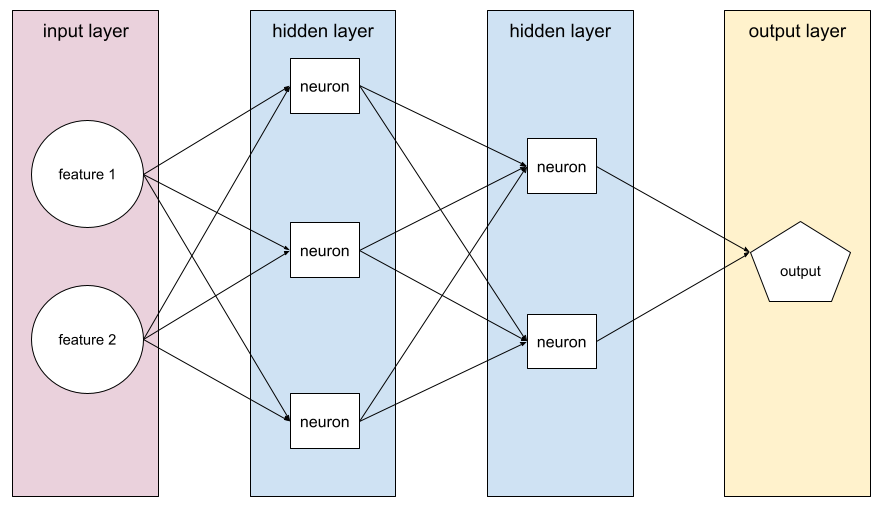
\includegraphics[width=\linewidth]{figs/NeuralNetwork.png}
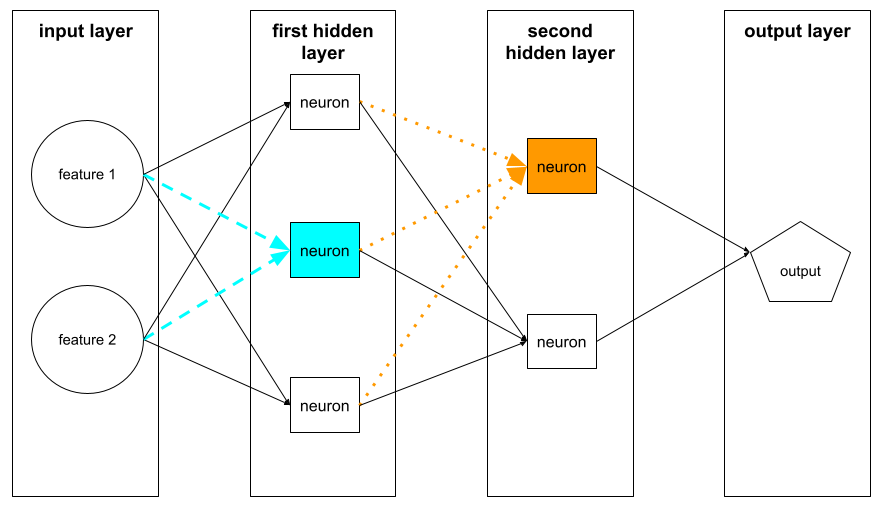
\includegraphics[width=\linewidth]{figs/Neurons.png}
\caption{A schematic deep NN with two hidden layers.
{\it Top}: Features in the input layer
are fed to neurons in the hidden layers, which eventually yield
a prediction in the output layer. {\it Bottom}: A schematic
highlighting what is fed into each neuron. Images taken 
from~\cite{google_ML}.}
\label{fig:neuralNet}
\end{figure}

\subsection{Neural networks}\label{sec:NN}

There are many, many strategies to construct an ML model.
A popular strategy is to construct a {\it neural network}\index{neural network}
(NN), which is shown schematically in \figref{fig:neuralNet}. 
A NN is organized into {\it layers}\index{layer}, which except\footnote{Or if you like
I suppose you could imagine the input layer performs the identity
transformation on the features.} for the input layer,
perform some transformation on information from the preceding layer. 
The {\it input layer}\index{layer!input} contains the features, and
the {\it output layer}\index{layer!output} yields the final predictions.

In between the input and output layers are 
{\it hidden layers}\index{layer!hidden} containing {\it neurons}\index{neuron}.
If there is more than one hidden layer, we call the NN a {\it deep}
NN\index{neural network!deep}\footnote{And sometimes if there is only one
layer but many neurons per layer, it is called {\it wide}\index{neural
network!wide}.}.
As a first step toward building a NN, one might imagine transforming
feature data using weighted sums. So for example 
the blue neuron in \figref{fig:neuralNet} (bottom), which I will
call $h_{12}$, indicating hidden layer 1 neuron 2, might take values
$x_1$ and $x_2$ from feature 1 and feature 2, respectively, and compute
\begin{equation}\label{eq:layer1}
h_{12} = w_{11}x_1+w_{12}x_2.
\end{equation}
Then the orange neuron would compute
\begin{equation}
h_{21} = w_{21}h_{11}+w_{22}h_{12}+w_{23}h_{13},
\end{equation}
with the output layer yielding
\begin{equation}
{\rm output} = w_{31}h_{21}+w_{32}h_{22}.
\end{equation}
Equation~\eqref{eq:layer1} focuses on on just one neuron. This can be succinctly
generalized to encapsulate all neurons in hidden layer 1; in particular
\begin{equation}
h_1=W x,
\end{equation} 
where $W=w_{ij}$ is the {\it weight matrix}\index{weight matrix}.

In this NN, the output can be written linearly in terms of the input $x_i$;
in other words, the NN models the labels as a linear function of the features.
The NN is characterized completely by the weights $w_{ij}$ and the connections
shown in the diagram. Note that each node in each layer depends on
every\footnote{This makes sense since it's the most
general strategy we could take. If a node in a preceding layer turns out
not to matter, a reasonable NN should compute the corresponding weight to be
zero. In principle you do not have to construct the NN in this way, and
so sometimes we say such NNs have {\it dense} or {\it fully connected}
layers\index{layer!dense}\index{layer!fully connected}.} input in the preceding layer.

The above NN clearly models labels as linear functions of features; on the other
hand, there is a wealth of phenomena that are more aptly understood as nonlinear
functions of input parameters, some of them highly so. In order to model
nonlinearity, a simple extension could be to feed the linear ansatz at each
neuron into some nonlinear function, called an {\it activation
function}\index{activation function}.  

At this stage I want to take a moment to discuss NN nomenclature and maybe
understand what inspired NNs to begin with. 
Based on its name, it clearly takes a cue from how
brains in animals work. Communication in brains is mediated by electrical
signals that travel from neuron to neuron. These electrical signals are
carried chemically by ions\footnote{There is some evidence
of electrical signals that travel through low-resistance pathways or
are influenced by extracellular electric fields~\cite{faber_two_2018}.},
and across the neuron's cell wall, there is an electric potential due to ions 
inside and outside the neuron. Moreover built into the cell wall are channels
that allow ions to flow in or out of the neuron. In the default or resting
state, these channels are closed, but when that potential difference reaches
some voltage threshold, a channel can open, allowing ions to flow easily
and reduce the potential difference. In a biological context, this
nexus of neurons is called a neural network\footnote{Therefore sometimes NNs
in the ML context are referred artificial neural networks.}, and hence
we can see that the network of what we call ``neurons" in an ML context
is an attempt to mimic brains in nature. The way channels open and close
 inspires not only the ``activation function" terminology but also many of 
the activation functions chosen in ML, which we will see often resemble 
step functions.

Okay let us return to constructing a nonlinear model using activation functions.
We modify hidden layers so that they instead do something like
\begin{equation}
h_{12} = A\left(w_{11}x_1+w_{12}x_2\right)
\end{equation}
for some activation function $A$. Popular choices include
$A(x)=\tanh(x)$, the {\it sigmoid}\index{sigmoid} function,
\begin{equation}
A(x)=\frac{1}{1+e^{-x}},
\end{equation}
the {\it rectified linear unit}\index{ReLU} (ReLU),
\begin{equation}
A(x)= \begin{cases}0 & x<0 \\ x & x \geq 0\end{cases},
\end{equation}
and the {\it leaky} ReLU\index{ReLU!leaky}, 
\begin{equation}
A(x)= \begin{cases}\alpha x & x<0 \\ x & x \geq 0\end{cases},
\end{equation}
for some small constant $\alpha$. Which activation function is best suited
for the task depends on the task at hand. Activation functions that output
in $[0,1]$ can be interpreted as probabilities, which may\footnote{For example
if the task of your NN is to classify images of dogs, it must be that
$\pr{\rm{dog}}+\pr{\rm{not dog}}=1$.} make sense
depending on your needs. The sigmoid function and $\tanh$ involve
exponentials, and hence may be slower to compute than ReLU. 
Finally, activation functions can be shifted adding a {\it bias}\index{bias}
in their arugment, which can be represented as a constant shift added
to weight produces like $Wx+b$. Adding a bias can be useful to e.g. change
activation thresholds, which may be necessary to make a model more accurate.

We now have constructed a relatively elementary, nonlinear NN to 
model labels as a function of features. How good of a model will this be?
It is in some sense mathematically guaranteed to be extremely good.
There are many {\it universal approximation theorems}\index{universal
approximation theorem} which guarantee that NNs converge to real-world
relationships. More precisely if we imagine our labels as a function $f$ of the
features and give some closeness criterion $\epsilon>0$, there exists some
number of neurons such that a NN approximates $f$ within $\epsilon$.
For example NNs with as few as one hidden layer and arbitrary bounded,
nonconstant activation function approximate well, provided there
are enough neurons~\cite{hornik_approximation_1991}.

All that remains for our simplistic example is the problem of determining
the weights $w_{ij}$. Once the weights are determined, we can give arbitrary
feature data $x_i$ and the NN will compute a corresponding label prediction. 
It is not hard to see that this is essentially a least-squares problem:
we will effectively ``fit" the NN using several examples.
In this context, one constructs some {\it loss} function\index{loss function},
which is analogous to $\chi^2$ in the least-squares approach.
We show the machine repeated examples, and it iteratively computes weights
that minimize the loss function. This process is called {\it
training}\index{training}. Just like with a standard fit, guesses for weights
are computed using well known algorithms such as the gradient descent.
This can be another consideration when picking an activation function, as
these algorithms may struggle to pick out weights for activation functions 
that vary little over large ranges.

It is common practice to take your original data, i.e. your original set of
examples, and organize them into subsets. There is a {\it training
set}\index{set!training}, a {\it validation set}\index{set!validation},
and a {\it testing set}\index{set!testing}. These sets are utilized in three
typical stages of building the ML model:
\begin{enumerate}
\item Training: You use the training set to compute the initial weights.
When the fitting procedure has visited every example once, we call
that an {\it epoch}\index{epoch}. In this stage, one may also subdivide
the training set into {\it batches}\index{batch}. Finally algorithms
like the gradient descent have an adjustable step size, in this
context called a {\it learning rate}\index{learning!rate}. Settings such 
as the number of epochs, the number of batches, or the learning rate 
are chosen by the user and will ultimately affect the
weights that are computed. These settings are sometimes referred to
as {\it hyperparameters}\index{hyperparameter}.
\item Validation:\index{validation} You loose the model on the 
validation set. There will
be some metric you use to determine whether the weights computed in
the training set are reasonable. At this stage, you still have the opportunity
to make adjustments to the ML model.
\item Testing:\index{testing} Finally you use the testing set to
ensure good performance of the tuned model.
\end{enumerate}


\begin{figure}
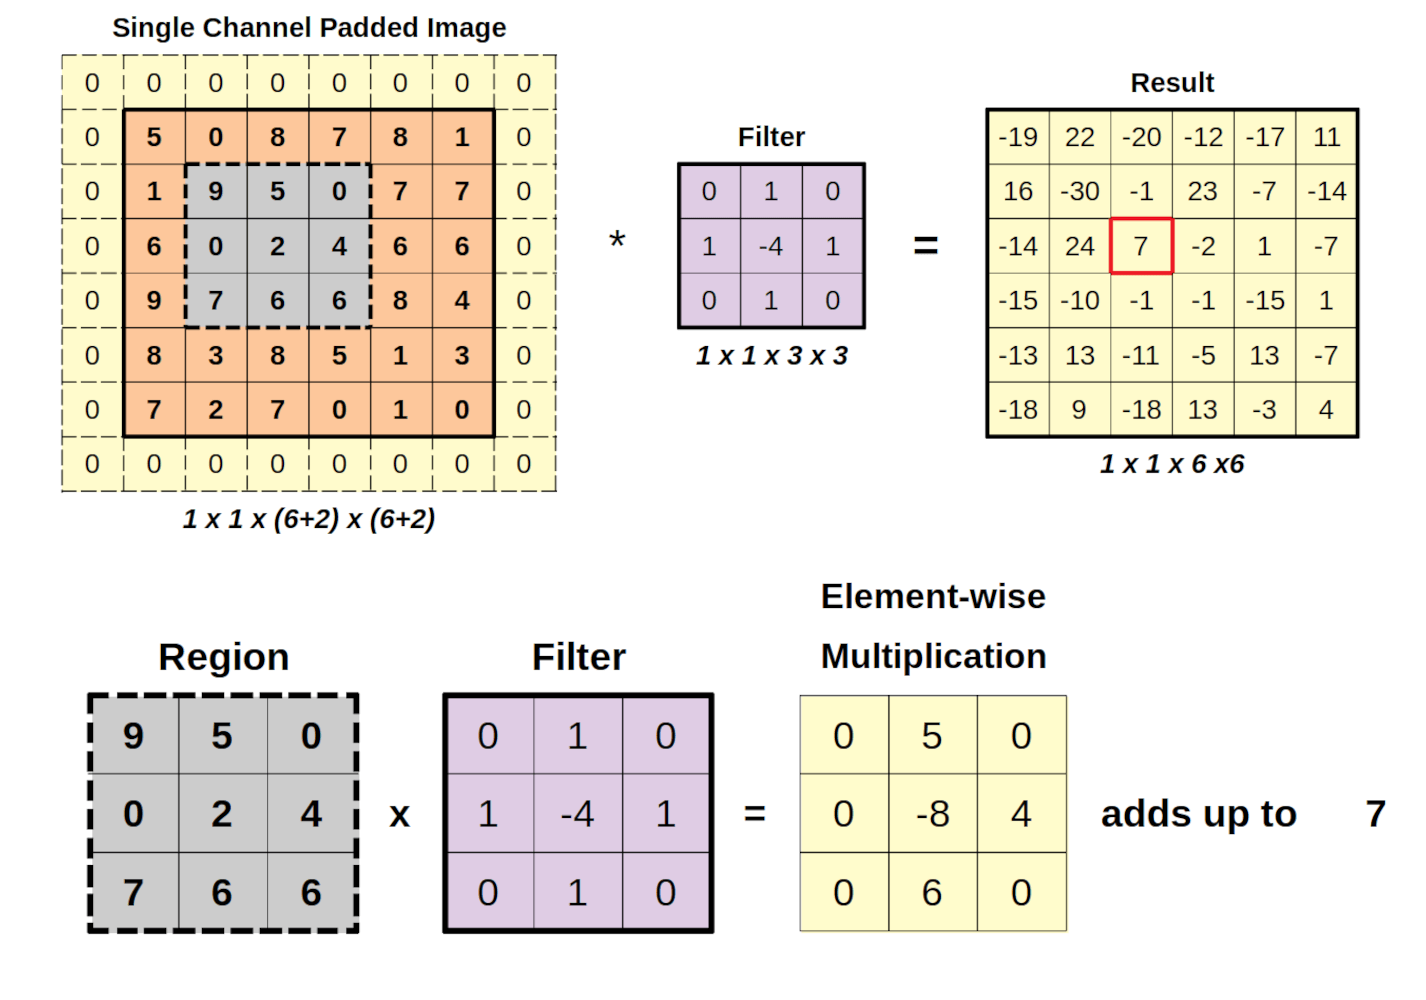
\includegraphics[width=\linewidth]{figs/CNN_filter.png}
\caption{An example convolution of a filter/kernel
of size $3\times 3$ with background pixels.
Image taken from Wikipedia~\cite{wikiCNN}.}
\label{fig:CNN}
\end{figure}

A {\it convolutional neural network}\index{neural network!convolutional} (CNN) 
adds an additional layer to the architecture, the 
{\it convolutional layer}\index{layer!convolutional}. CNNs are employed usually 
in tasks of image recognition; hence we imagine a training process that scans
over some set of pixels, with the goal of trying to extract some features from
them.

The convolutional layer is what carries out this task. It introduces a 
{\it filter}\index{filter} or {\it kernel}\index{kernel}. For a 2-$d$ image, the
kernel is a 2-$d$ grid, typically of size $3\times 3$, within which one
specifies some values in the grid like 0 or 1. One then performs an inner
product of the kernel with the pixels, as shown in \figref{fig:CNN}. This maps
the original set of pixels to a smaller, coarse-grained set of 
pixels\footnote{This is similar in spirit to a renormalization-group transform.},
thereby lowering the information sent to the next part of the layer.
Depending on the task at hand, the kernel size, the contents of the kernel,
and the {\it stride}\index{stride}, a hyperparameter specifying 
the number of pixels the kernel moves before
performing the next inner product, must be adjusted.

\subsection{Unsupervised learning}

Up to now we have discussed ML examples of 
{\it supervised learning}\index{learning!supervised},
where someone has to give some information to the ML model, in particular the
labels on the training data. By contrast in {\it unsupervised}\index{learning!unsupervised}, 
or {\it self-supervised}\index{learning!self-supervised} learning we provide no
labels, and instead sic some
ML model on a set of data, allowing the model itself to discover any patterns.

There are many strategies to achieve this. One strategy is to map each data
point to $\R^n$. This target space is sometimes called a 
{\it latent space}\index{space!latent}
or {\it embedding space}\index{space!embedding}.
The ML model can then try to measure distances between each
point in $\R^n$ to discover clusters. These are examples of {\it clustering
algorithms}\index{clustering algorithm}.
Alternatively after such a mapping, one could use 
{\it principal component analysis}\index{principal component analysis} (PCA).
For PCA, one tries to find a set of independent directions in $\R^n$ spanning
the data. If we imagine the data as arranged in an ellipsoid, PCA tries to
find its principal axes.


Another useful algorithm for learning features is called an
{\it autoencoder}\index{autoencoder}. It contains a hidden layer
$c$ called an {\it encoder}\index{encoder} that represents the input $x$
by $c(x)$. There is also a {\it decoder}\index{decoder} $d$ which ought to satisfy
\begin{equation}\label{eq:autoencoder}
x=d(c(x)).
\end{equation}
In principle there are many useless transformations
$c$ that will not teach us anything new about the data. What we would like is to
constrain $c$ in such a way that \equatref{eq:autoencoder} is approximate,
with the hope that $c$ will expose the data's most salient features.

One way of doing this is to enforce that $c(x)$ has a smaller\footnote{A CNN
also creates a new data set of lower dimension than the input through
convolution with the kernel. Rather than specifying the dimensional reduction
should be a convolution, the autoencoder is asked to find the transformation
itself.} dimension than $x$. Such autoencoders are said to be
{\it undercomplete}\index{undercomplete}. With a mind toward 
\equatref{eq:autoencoder}, the learning process consists of minimizing
a loss function $L(x,d(c(x)))$ that penalizes $d(c(x))$ for being
too different from $x$. If the decoder is linear and $L$ is
the mean-squared error, the undercomplete autoencoder will learn to
span the same space as PCA~\cite{Goodfellow_2016}. 

\begin{figure}
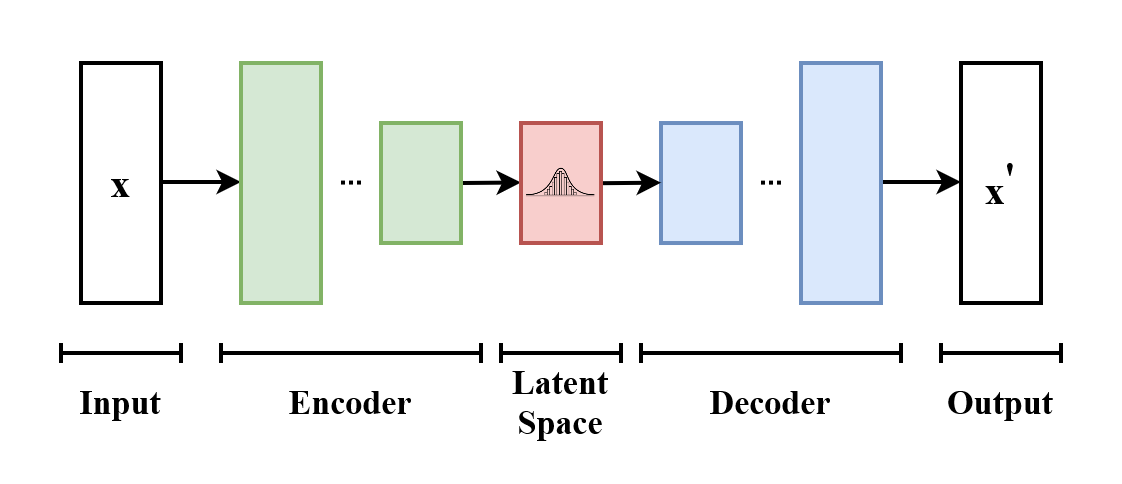
\includegraphics[width=\linewidth]{figs/VAE.png}
\caption{A schematic variational autoencoder.
Image taken from Wikipedia~\cite{wikiVAE}.}
\label{fig:VAE}
\end{figure}

Depending on choices like the mapping $c$, the desired dimensionality of $c(x)$,
and so on, an autoencoder may in some sense learn too well. What this means in
practice is that the original data are too closely mimicked, and hence no
interesting features of the data can be extracted. Generally speaking there
are many strategies to avoid such overfitting\index{overfitting}. 
In the case of autoencoders,
one can employ a {\it variational autoencoder}\index{autoencoder!variational}.
In this algorithm, the output of the code is used to create a probability
distribution; for example you could compute the mean and variance of $c(x)$ and
create a Gaussian distribution $f$ from that. Then instead of passing $c(x)$
directly to $d$, the machine draws a sample from $f$ which is then passed to
$c$. A schematic of this process is shown in \figref{fig:VAE}.

Another example of an unsupervised\footnote{Contrastive learning can also
be used in supervised contexts. In the parlance of the following discussion,
in the supervised case, one would label the example $e$ and incorporate
that label in the loss function.} algorithm is called {\it contrastive
learning}\index{contrastive learning}. Here one starts with an example $e$,
then applies small transformations to $e$ creating new examples, say $e'$ and
$e''$. This process of creating these new examples is called {\it data
augmentation}\index{data augmentation}\footnote{Data augmentation can be
employed also in other ML models.}. 
In the context of image classification,
common transformation include cropping the image, changing its color, flipping
it, rotating it, and so on. 
After embedding $e'$ and $e''$ in the latent space, one designs loss functions
that punish points in the space that came from different original examples $e$.

\subsection{Some details about training}

In \secref{sec:NN}, we explained that training can be cast as a least-squares
problem. The loss function is the to-be-minimized function, and its minimum
in weight space can be found e.g. using gradient descent.

As a reminder, gradient descent works by computing partial derivatives of 
a function with respect to its parameters. In the context of least-squares, that
means the algorithm proceeds along the gradient of the $\chi^2$ with respect
to the fit parameters; in the context of machine learning, we proceed along the
gradient of the loss function with respect to its weights. A modern strategy for
computing partial derivatives is {\it automatic differentiation}\index{automatic
differentiation}.

The idea behind automatic differentiation is relatively simple. Consider a composite
function $f(g(h(x,y)))$. Suppose you already understand how to take a derivative
of the functions $f$, $g$, and $h$. You can imagine $f$, $g$, and $h$ represent
some single elementary operation, say $f$ represents $\sin$, $g$ represents
$\cos$, and $h$ represents multiplication. If you code up how to take a generic
derivative for each of those three operations, you can take the derivative of
$f\circ g\circ h$, and in fact, you can take a derivative of an arbitrary
composition of $f$, $g$, and $h$. Automatic differentiation tries to leverage
that every computer operation carries out a sequence of arithmetic operations
and elementary functions. One obtains ``exact" results without having to go
through a slow, symbolic manipulation.

When carrying out gradient descent for the loss function, one uses {\it
backpropagation}\index{backpropagation}. Backpropagation uses automatic
differentiation to compute these partial derivatives layer by layer starting
from the first layer. It employs tricks to improve efficiency, for example
finding ways to avoid redundant calculations in intermediate steps of the chain
rule.

\subsection{Judging ML model performance}

In \secref{sec:NN} we sketched a three-step process for tuning a NN.
Here we wish to discuss aspects of this process in detail, for example
elucidating the role of the testing phase compared to the validation phase.

The point of training is that the model describes data better and better as
training progresses. As a consequence, one should expect that the loss function
decreases and roughly converges with increasing epochs. This can be a metric of
performance for ML models.

Again, a common goal of constructing NNs is to model labels as a function of
features. How well the NN models the data depends on what one feeds to it during
training, and again thinking about the connection to least-squares problems,
one can imagine fitting the weights and biases to the training data. Just like
with ordinary fitting, one can {\it overfit}\index{overfitting} the data: This
often amounts to taking fluctuations in training data too seriously, baking structure
into the model that is either irrelevant or not really there, stemming instead
from e.g. statistical noise. Just as in ordinary least-squares problems,
a model is more susceptible to overfitting when there are too many fit
parameters relative to the amount of training data. 
Overfit models will label the training data
extremely well, but having ``learned" irrelevant features and/or noise in the
training data, will generally not perform well when presented with completely
new data. In ML parlance, one might say that the overfit model does not
{\it generalize}\index{generalization} well. Another drawback to overfitting
manifests for models whose output layers are to be interpreted as probabilities.
Overfitted NNs may find a high likelihood that a datum belongs to a particular
label while also getting the label wrong. In this context, overfitting
translates to a problem of {\it overconfidence}\index{overconfidence}.

As suggested by the above paragraph, one way to check if a model has been
overfitted is to see how well it generalizes. One way to do this is to set aside
another set of data to see if the trained, validated model performs well in a
new situation. This a motivation for the testing stage. A model that performed
well during validation but poorly during testing may suffer from overfitting.
Another check is to compare the dependence of the loss function against the
number of epochs between the training and validation sets. In this context, a
sign of overfitting can be that the validation loss curve diverges with increasing 
epochs compared to the training loss curve.

Just as with least-squares approaches, overfitting can be combatted by
penalizing model complexity. For example in the context of ordinary
least-squares fits, model quality is sometimes judged using various information
criteria, which often add to the $\chi^2$ a penalty that increases with
increasing number of fit parameters. Thus to prevent overfitting, instead of
minimizing a bare loss function, one may seek to minimize
\begin{equation}
{\rm loss}+\lambda~{\rm regularization},
\end{equation}
with the latter {\it regularization}\index{regularization} term quantifying the
overfitting and $\lambda$ an adjustable parameter to give more or less weight to
this term compared to the loss.

A simple and popular choice of regularization is the $L_2$ 
{\it regularization}\index{regularization!L2}. Here the regularization is computed as
the sum of squares of the weights, which punishes weights that are away from
zero. For each weight, this forces the machine to make a decision how important
that weight is: Weights that decrease the loss function only very little will
ultimately be punished by the regularization. In that sense, the model is forced
to focus on the most important weights only.

Another popular choice is\index{regularization!dropout} {\it dropout
regularization}~\cite{srivastava_dropout_2014}. In this scheme, every neuron of
either the input or hidden layer is removed, along with its connections, with
probability $p$. This procedure helps combat {\it
co-adaptation}\index{co-adaptation}, which is ML jargon that refers to neurons
in hidden layers having large correlations. The 
resulting {\it thinned network}\index{neural network!thinned}
represents a draw from a sample of all possible neural networks. Weights must be
normalized with the dropout probability $p$ in order to ensure the weights keep
the same scale relative to each other. Dropout can lead to lower test classification 
error compared to $L_2$ regularization~\cite{srivastava_dropout_2014}.


\bibliographystyle{unsrtnat}
\bibliography{bibliography}
